\documentclass[11pt]{article}

% load some asm stuff -
\usepackage{amssymb}
\usepackage{amsmath}
\usepackage{amsthm}
%\usepackage{palatino,lettrine}
\usepackage{fancyhdr}
\usepackage{epsfig}
\usepackage[round,comma,sort]{natbib}
\usepackage{simplemargins}
\usepackage{setspace}
\usepackage[margin=0pt,font=small,labelfont=bf]{caption}

\bibliographystyle{plos2009}

% Set the size
%\textwidth = 6.75 in
%\textheight = 9.75 in
%\oddsidemargin = 0.0 in
%\evensidemargin = 0.0 in
%\topmargin = 0.01 in
%\headheight = 0.0 in
%\headsep = 0.25 in
%\parskip = 0.15in
\doublespace

\setallmargins{1in}

\newtheorem{example}{Example}[section]
\newtheorem{thm}{Theorem}[section]
\newtheorem{property}{Property}[section]

\theoremstyle{definition}
\newtheorem{defn}[thm]{Definition}

\makeatletter
\renewcommand\subsection{\@startsection
	{subsection}{2}{0mm}
	{-0.05in}
	{-0.5\baselineskip}
	{\normalfont\normalsize\bfseries}}
\renewcommand\subsubsection{\@startsection
	{subsubsection}{2}{0mm}
	{-0.05in}
	{-0.5\baselineskip}
	{\normalfont\normalsize\itshape}}
\renewcommand\paragraph{\@startsection
	{paragraph}{2}{0mm}
	{-0.05in}
	{-0.5\baselineskip}
	{\normalfont\normalsize\itshape}}
\makeatother
\linespread{1.2}

\fancypagestyle{proposal}{\fancyhf{}%
	\fancyhead[RO,LE]{\thepage}%
	\fancyhead[LO,RE]{ChE 525 Biochemical Balances and Black Box Models of Cells}%
	\renewcommand\headrulewidth{1pt}}
\pagestyle{proposal}

% Single space'd bib -
\setlength\bibsep{0pt}

\renewcommand{\rmdefault}{phv}\renewcommand{\sfdefault}{phv}

%\newboxedtheorem[boxcolor=black, background=gray!5,titlebackground=orange!20,titleboxcolor = black]{color_box_example}{Example}{test}

% Change the number format in the ref list -
\renewcommand{\bibnumfmt}[1]{#1.}

% Change Figure to Fig.
\renewcommand{\figurename}{Fig.}

%Joycelyn Chan, Joshua Lequieu, Michael Paull, Chidanand Balaji, Ryan Tasseff
%Our derivation follows closely the earlier development of Fredrickson \citep{Fredrickson:1976fk}.

% Begin ...
\begin{document}

%\begin{titlepage}
{\par\centering\textbf{\Large Biochemical Engineering Balances and Black Box Models of Cells}}
\vspace{0.2in}
{\par \centering \large{Jeffrey D. Varner$^{*}$}}
\vspace{0.05in}
{\par \centering \large{School of Chemical Engineering$^{*}$}}
{\par \centering \large{Purdue University, West Lafayette IN 47907}}
\vspace{0.1in}
{\par \centering \small{Copyright \copyright\ Jeffrey Varner 2016. All Rights Reserved.}}\\

%\end{titlepage}
\date{}
\thispagestyle{empty}

\setcounter{page}{1}

%material and energy balances around the different processes cells do. For example, understanding how the abundance of raw materials in a bioreactor influences
%cell growth, or the production of valuable protein or small molecule products requires a materials balances around the major components of the system.
%The production of valuable small molecule or protein products requires large connected intracellular reaction networks that produce or consume energy.
%Thus, to understand the operation of biochemical systems and ultimately to manipulate them for societal gain,

\section*{Introduction}
The basic building block of any biomolecular process is a cell. Cells are biological agents which consume nutrients, and process these nutrients to make valuable products,
waste products and more cells. The chemical transformation of nutrients e.g., sugar to valuable products such as \textit{proteins} or organic molecules uses a vast
network of coupled chemical reactions collectively called \textit{metabolic~pathways}.
Cells differ in their size, shape, behavior and complexity. However, they all share the common thread of requiring nutrients to survive, and many of the
pathways that process nutrients are conserved from the simplest bacteria to the most complex cells in our bodies.
We can grow cells and use them to make products of interest in special chemical reactors called \textit{bioreactors}.
To understand how cells function in bioreactors, and ultimately how to manipulate them for societal benefit, we must first understand how to apply engineering principles such as conservation of
mass and energy to biological systems. Toward this goal, we'll start by reviewing basic material balance concepts and use these concepts to write balance equations around \textit{extracellular} nutrients
(nutrients outside of the cell). Second, we'll begin to think about how cells process extracellular nutrients, and how to write material balances around cells in bioreactors.

\subsection*{Total macroscopic mass and mole balance equations.}
\begin{figure*}[!ht]\centering
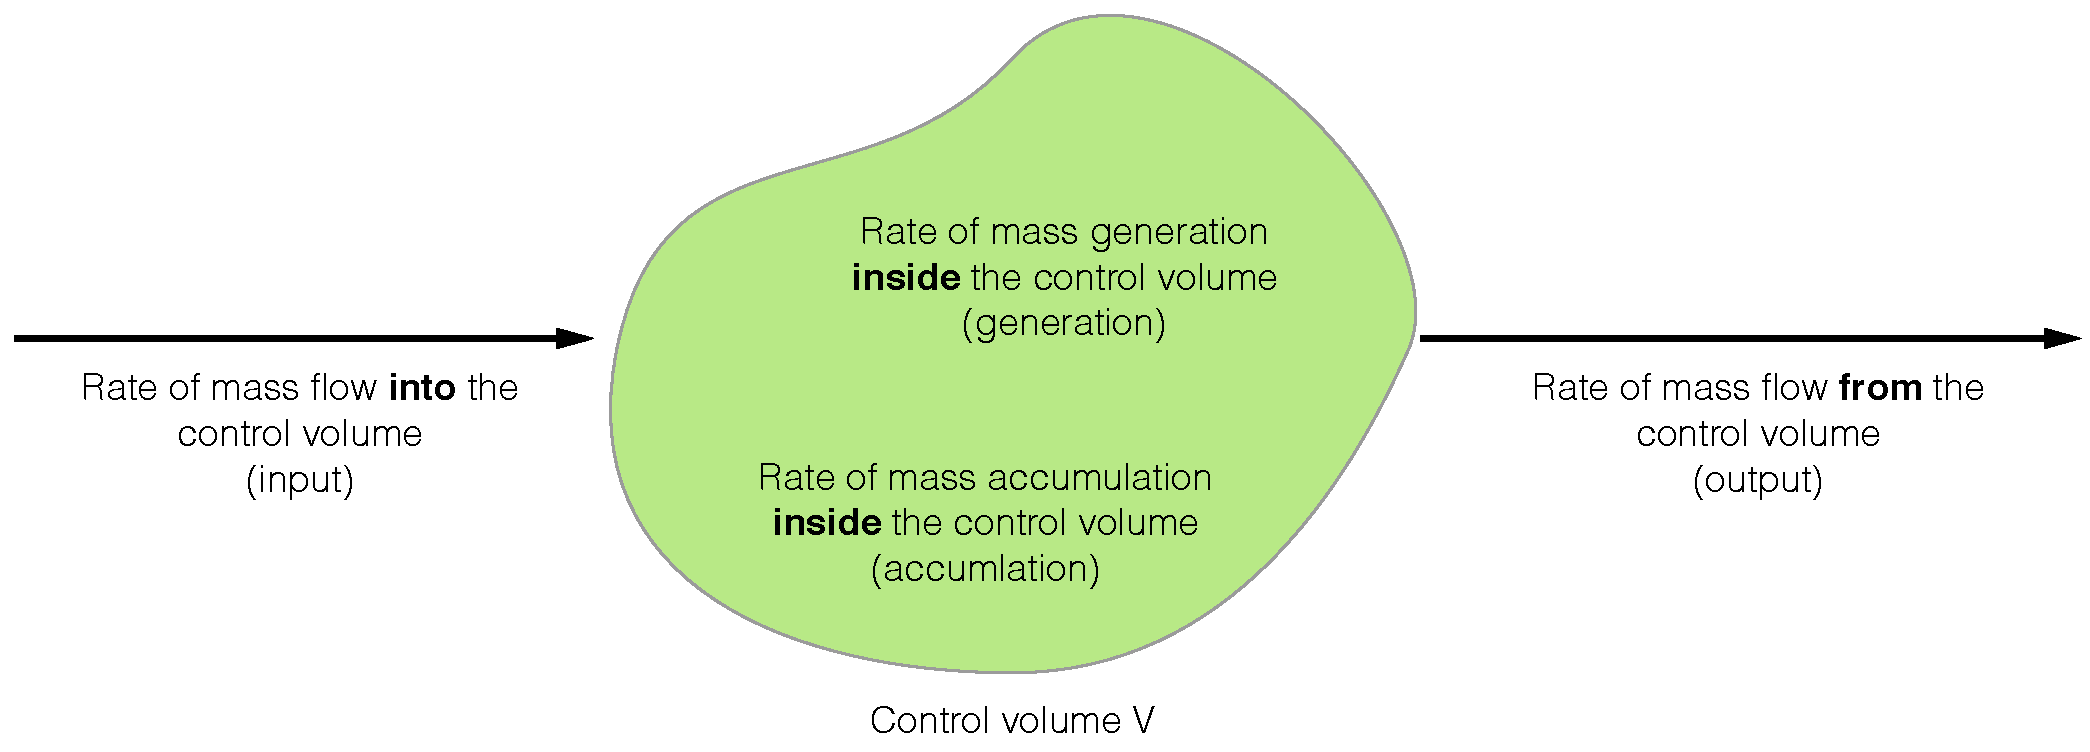
\includegraphics[width=1.0\textwidth]{./figs/Control-Volume.pdf}
\caption{Schematic of an idealized control volume V. Total macroscopic material balance equations consist of four types of terms.
Material flow into and from the control volume, material generation inside the control volume and material accumulation inside the control volume.
The abundance of material can be measured using both a mass or mole basis.}\label{fig-control-volume}
\end{figure*}

Consider an idealized control volume (Fig. \ref{fig-control-volume}).
The total macroscopic material balance around the control volume contains four terms, flow in, flow out, generation ($\dot{m}_{gen}$) and accumulation ($\dot{m}_{acc}$):
\begin{equation}\label{eqn-total-mass}
	\sum_{s~=~1}^{\mathcal{S}}v_{s}\dot{m}_{s} + \dot{m}_{gen} = \dot{m}_{acc}
\end{equation}
The summation term:
\begin{equation}
\sum_{s~=~1}^{\mathcal{S}}v_{s}\dot{m}_{s}
\end{equation}
describes the net rate of material flow into and from the control volume, where $\dot{m}_{s}$ denotes the mass flow
\emph{rate} of stream s (typical units of kg/hr) and $\mathcal{S}$ denotes the total number of streams. The quantities
$v_{s}$ are direction parameters. We'll use the convention that streams entering the control volume have
positive direction parameters ($v_{s} = 1$), while streams exiting the control volume ($s^{*}$) have negative direction parameters ($v_{s^{*}} = -1$),
The term $\dot{m}_{gen}$ describes the \emph{rate} of total mass generation inside the control volume,
while $\dot{m}_{acc}$  describes the \emph{rate} of total mass accumulation inside the control volume.
For biochemical processes, total mass is conserved (it is neither created or destroyed), thus $\dot{m}_{gen} = 0$.

Just like total mass balances, we can also write a balance equation around the \textit{total} number of moles in a process.
Total mole balances have the same four types of terms, input, output, accumulation and generation and take the form:
\begin{equation}
\sum_{s = 1}^{\mathcal{S}}v_{s}\dot{n}_{s}+\dot{n}_{gen} = \dot{n}_{acc}
\end{equation}where $\dot{n}_{s}$ denotes the rate of transport of total moles in stream $s$ (mol/time), $\dot{n}_{gen}$ denotes the rate of generation of total moles in a process (mol/time),
and $\dot{n}_{acc}$ denotes the rate of accumulation of moles inside the process (mol/time), and $v_{s}$ denotes our direction parameter.
However, unlike total mass balances, the generation term in mole balances can be non-zero ($\dot{n}_{gen}\neq{0}$) in some cases (especially for reactive systems).

Lastly, we can also write species balances using moles. For example, the balance around species k is given by:
\begin{equation}
	\sum_{s = 1}^{\mathcal{S}}v_{s}\dot{n}_{s}x_{k,s}+\dot{n}_{k,gen}=  \dot{n}_{k,acc}\qquad{k=1,2,\hdots,\mathcal{M}}
\end{equation}where $x_{k,s}$ denotes the mole fraction of species k in stream s.
If stream s is a vapor or gas, we use the symbol $y_{k,s}$ to denote the mole fraction of species k in stream s.
We can also express mole-based species balances in terms of the concentration of species k ($C_{k}$) in the control volume:
\begin{equation}\label{eqn:general-species-mole-balance}
\sum_{s = 1}^{\mathcal{S}}v_{s}F_{s}C_{k,s} + \dot{n}_{k,gen} = \frac{d}{dt}\left(C_{k}V\right)\qquad{k=1,2,\hdots,\mathcal{M}}
\end{equation}where $F_{s}$ denotes the volumetric flow rate (L/hr) in stream $s$, $C_{k,s}$ denotes the concentration of species k in stream s, and $V$ denote the volume (L) of the control volume.
We can write a balance of the form shown in Eqn. \eqref{eqn:general-species-mole-balance} for each of the $\mathcal{M}$ species in the bioreactor.

\subsubsection*{Aside: Where does the well mixed assumption come into play?}
The well-mixed assumption is hidden in the derivation of Eqn \eqref{eqn:general-species-mole-balance}!
If we step back, the accumulation and reaction terms are actually given by:
\begin{equation}
\dot{n}_{k,acc} = \frac{d}{dt}\int_{V}C_{k}dV\qquad{k=1,2,\hdots,\mathcal{M}}
\end{equation}where $C_{k}$ denotes the general concentration [abundance/volume] of species $k$ in control volume V.
The generation term can also be written in integral form:
\begin{equation}\label{eqn-generation}
	\dot{n}_{k,gen} = \int_{V}\left(\sum_{g}\sigma_{kg}r_{g}\right)dV\qquad{k=1,2,\hdots,\mathcal{M}}
\end{equation}where $r_{g}$ denotes the rate of chemical reaction $g$ [abundance/volume-time] occurring in volume V.
The summation is done over all possible reactions occurring in the control volume.
Putting everything together gives:
\begin{equation}\label{eqn-species-mass-balance-no-assumptions}
	\frac{d}{dt}\int_{V}C_{k}dV = \sum_{s = 1}^{\mathcal{S}}v_{s}F_{s}C_{k,s} + \int_{V}\left(\sum_{g \in \mathcal{R}}\sigma_{kg}r_{g}\right)dV\qquad{k=1,2,\hdots,\mathcal{M}}
\end{equation}
The integration in Eqn \eqref{eqn-species-mass-balance-no-assumptions} is over the control volume V.
However, if we assume that concentration does not vary over the volume V (the well mixed assumption), then the integrals can be simplified e.g.,
\begin{equation}
		\frac{d}{dt}\int_{V}C_{k}dV \simeq \frac{d}{dt}\left(C_{k}V\right)
\end{equation}which gives the material balance given by Eqn \eqref{eqn:general-species-mole-balance}.

\subsection*{Well mixed extracellular material balance equations.}
To analyze the behavior of cells in a bioreactor, we need to write material balances around nutrients, cells, metabolic products and the volume of media in the bioreactor.
For bioreactors we'll exclusively use mole-based units, however, other mass-based units systems can be found in the biochemical literature.
Let's begin writing our balances by expanding the generation term in the general mole-based species balance given in Eqn \eqref{eqn:general-species-mole-balance}:
\begin{equation}
\dot{n}_{j,gen} = \left(\sum_{r}^{\mathcal{R}}\sigma_{jr}\hat{r}_{r}\right)V+\left(\sum_{k}^{\mathcal{T}}\tau_{j,k}q_{k}\right)XV
\end{equation}We have two sets of reaction terms, the first describes $\mathcal{R}$ chemical reactions that can occur in the absence of cells (in the bulk fluid in the reactor), while the second
describes those $\mathcal{T}$ reactions that occur because of cells (cell-associated reactions). For bulk fluid phase reactions, $\sigma_{jr}$ denotes the stoichiometric coefficient governing species j in reaction r;
if $\sigma_{jr}<0$ species j is \textit{consumed} by reaction r, if $\sigma_{jr}>0$ species j is \textit{produced} by reaction r and if $\sigma_{jr}=0$ species j is not connected with reaction r.
The quantity $\hat{r}_{r}$ denotes the reaction rate per unit volume for reaction r (mmol/L-hr).
Similarly, for the cell-associated reaction terms, $\tau_{j,k}$ denotes the stoichiometric coefficient describing how species j is connected with cell-associated reaction k.
Reactions associated with cells have a unique unit system called \textit{specific~units} which means we write all quantities per unit cell abundance (grams dry weight, or mmol of cells).
Thus, $q_{k}$, the kth cell-associated reaction rate, has units of mmol/mmol-hr or mmol/gdw-hr etc. Substituting our reaction terms into Eqn \eqref{eqn:general-species-mole-balance} gives:
\begin{equation}\label{eqn:general-balances}
\frac{d}{dt}\left(C_{j}V\right) = \sum_{s}^{\mathcal{S}}v_{s}F_{s}C_{j,s} + \left(\sum_{r}^{\mathcal{R}}\sigma_{jr}\hat{r}_{r}\right)V+\left(\sum_{k}^{\mathcal{T}}\tau_{j,k}q_{k}\right)XV \qquad j=1,2,\dots,\mathcal{M}
\end{equation}where $\mathcal{M}$ denotes the number of \textit{metabolites}, $X$ denotes the cellmass level in the reactor (gdw/L or mmol/L), and $V$ denotes the working volume (L) of the reactor.
Similarly, the cellmass balance is given by:
\begin{equation}\label{eqn:general-cellmass-balances}
\frac{d}{dt}\left(XV\right) = \sum_{s}^{\mathcal{S}}v_{s}F_{s}X_{s}+\left(\mu - k_{d}\right)XV
\end{equation}where $\mu$ denotes the \textit{specific~growth~rate} of cells, (hr$^{-1}$) and $k_{d}$ denotes the cell death constant (hr$^{-1}$).
Lastly, both the cellmass and metabolite balances involve the volume $V$ which is governed by:
\begin{equation}
\frac{dV}{dt} = \sum_{s~=~1}^{\mathcal{S}}v_{s}\frac{\rho_{s}}{\rho}F_{s} - \frac{V}{\rho}\frac{d\rho}{dt}
\end{equation}
Putting all three types of equations together, expanding all derivatives and dividing both sides of the extracellular metabolite and cellmass balances by the volume gives:
\begin{eqnarray}\label{eqn-metabolite-dilution-dynamic}
	\frac{dC_{j}}{dt} &=& \sum_{s~=~1}^{\mathcal{S}}v_{s}D_{s}C_{j,s} + \left(\sum_{r~=~1}^{\mathcal{R}}\sigma_{jr}\hat{r}_{r}\right) + \left(\sum_{k~=~1}^{\mathcal{T}}\tau_{j,k}q_{k}\right)X  - \frac{C_{j}}{V}\frac{dV}{dt}\qquad j=1,2,\dots,\mathcal{M}\\
	\frac{dX}{dt} &=& \sum_{s~=~1}^{\mathcal{S}}v_{s}D_{s}X_{s}+\left(\mu - k_{d}\right)X - \frac{X}{V}\frac{dV}{dt}\\
	\frac{dV}{dt} &=& \sum_{s~=~1}^{\mathcal{S}}v_{s}\frac{\rho_{s}}{\rho}F_{s} - \frac{V}{\rho}\frac{d\rho}{dt}
\end{eqnarray}where the quantity $D_{s}$,  called a \textit{dilution~rate} (hr$^{-1}$), is given as:
\begin{equation}
	D_{s} \equiv \frac{F_{s}}{V}\qquad s=1,2,\dots,\mathcal{S}
\end{equation} The cellmass, metabolite and volume balances are a coupled system of $\mathcal{M}+2$ nonlinear ordinary differential equations,
which depending upon the functional forms of the specific growth, death and uptake rates, has no analytic solution.
However, these equations can be easily solved numerically using common algorithms included in packages and languages such as MATLAB or Python.

\subsection*{Black box models of growing cells.}
Intracellular metabolic pathways convert extracellular nutrients, for example sugar, oxygen or nitrogen etc into cells, valuable products and waste products.
When we write balances describing the abundance of sugar, nitrogen or other metabolic inputs we should include descriptions of the metabolic pathways in our balances equations.
However, exhaustively modeling metabolic pathways is difficult; metabolic pathways consist of thousands of coupled chemical reactions, occurring simultaneously inside growing cells.
Thus, it is currently only feasible to completely model metabolism (the process of the breakdown of raw materials and construction of finished products)
for very simple organisms \citep{Karr:2012ve}. Instead, we'll make a simplifying assumption and treat cells as black boxes which consumes nutrients, produce more cells, and metabolic products (later, we'll relax this assumption). Consider the schematic of a simple cell shown in Fig. \ref{fig-simple-cells}.

\begin{figure*}[!ht]\centering
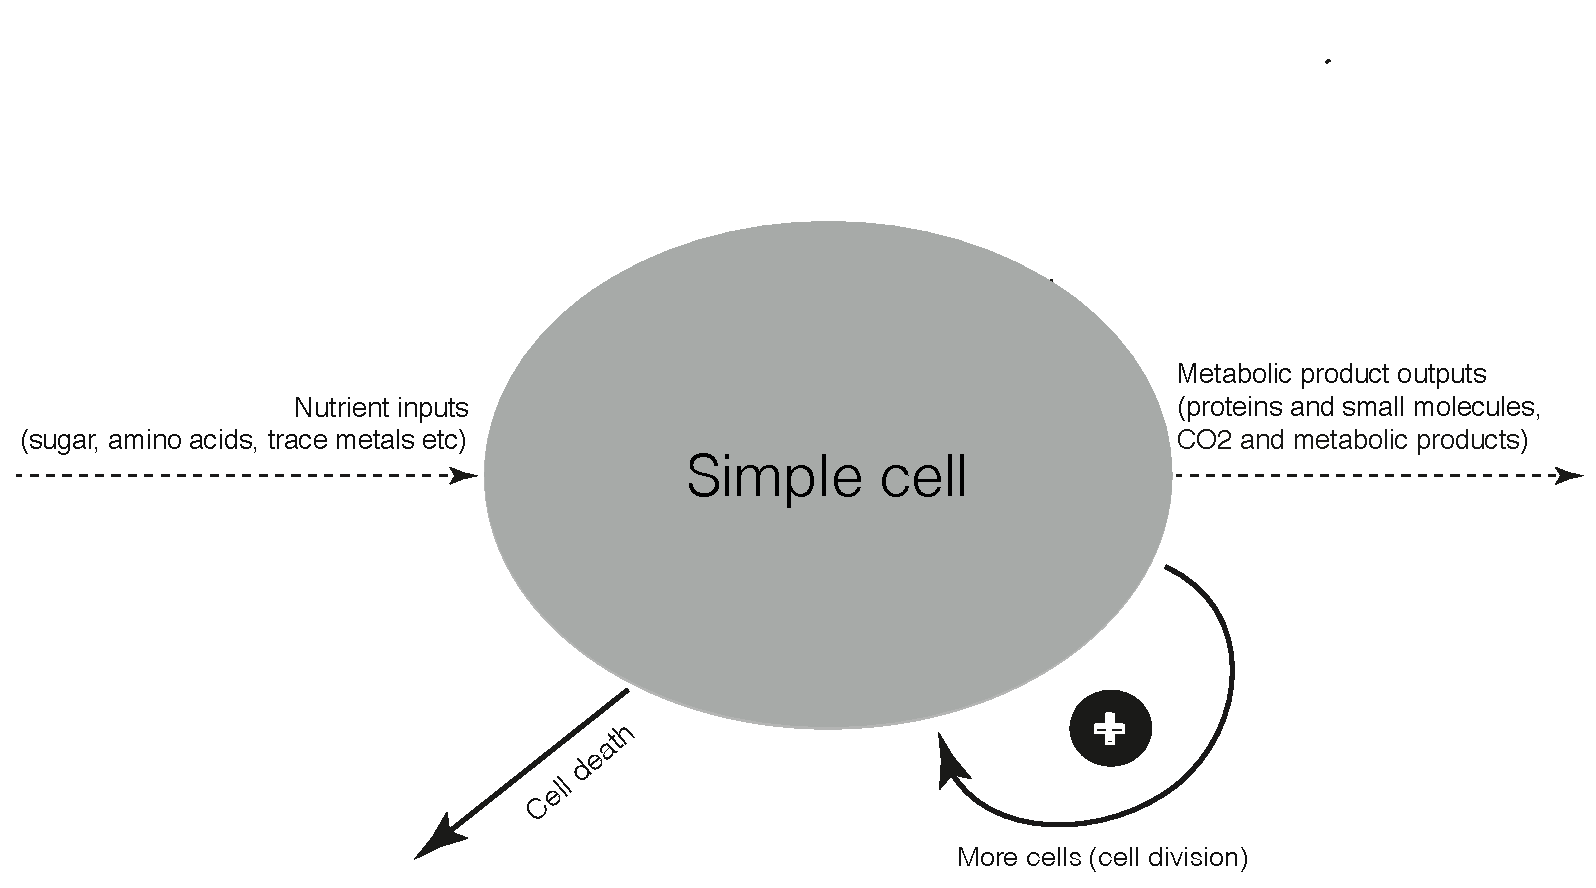
\includegraphics[width=0.9\textwidth]{./figs/SchematicSimpleCells-1-6-15.pdf}
\caption{Schematic of simple cells. Simple cells consume nutrients (carbon, nitrogen, etc), and process them to make metabolic products, waste products and more cells.
The dashed arrows denote catalytic behavior that simple cells do while the solid arrows indicate reactions that change the abundance of cells in a bioreactor. }\label{fig-simple-cells}
\end{figure*}

\noindent Simple cells consume nutrients $S_{1},S_{1},\hdots,S_{N}$ to produce products $P_{1},P_{2},\hdots,P_{M}$ and cells $X$.
In reality, this conversion involves many chemical reactions, however for now lets lump all of these into a single pseudo reaction:
\begin{equation}\label{eqn-growth-rate}
\sum_{i=1}^{N}a_{i}*S_{i} + X \longrightarrow n*X + \sum_{j=1}^{M}b_{j}*P_{j}
\end{equation}where $a_{i},b_{j}$ and $n$ are stoichiometric coefficients.
The stoichiometry of this pseudo reaction is described by a set of special \emph{non-constant} coefficients called yield coefficients, given the symbol $Y$.
Yield coefficients are a special type of stoichiometric coefficient that relate the consumption or production of a nutrient or product to cell growth.
For example, if species $j$ were a nutrient, $Y_{X/j}$ would quantify how much $j$ was consumed to product a unit of cells, or:
\begin{equation}
	Y_{X/j} \equiv -\frac{\Delta X}{\Delta C_{j}}
\end{equation}
In the general case, yield coefficients are \textit{not~constant} (we'll see examples of this later) and must be measured from experimental data,
or calculated using theoretical tools such as flux balance analysis (FBA) \citep{Orth:2010uq}.

\subsubsection*{What are the $\tau_{*}$ and $q_{*}$ in the general balances?}
The $\tau_{*}$ and $q_{*}$ terms that appear in the extracellular species balances describe the stoichiometry and specific rate of consumption or production (mmol/gdw-L) of
extracellular metabolites by simple cells. Lets assume that $\tau_{*} = -1$ for nutrients, while $\tau_{*} = 1$ for products.
We can then relate the specific uptake rate of nutrients to the specific growth rate of simple cells, and the cellmass yields using the Pirt equation \citep{Pirt:1965aa}:
\begin{equation}
q_{k} = \frac{1}{Y^{*}_{X/k}}\mu+m_{k}\qquad{k\in\left\{nutrients\right\}}
\end{equation}where $Y^{*}_{X/k}$ is the \emph{true} biomass yield on nutrient k, and $m_{k}$ denotes the maintenance utilization of nutrient k. Similarly, we can use the
Luedeking and Piret equation \citep{Luedeking:2000aa} to relate the specific rate of product formation to the specific growth rate:
\begin{equation}
q_{j} = \frac{1}{Y^{*}_{X/j}}\mu+\theta_{j}\qquad{j\in\left\{products\right\}}
\end{equation}where $Y^{*}_{X/j}$ denotes the true product yield, and $\theta_{j}$ denotes the non-growth associated production of product j.

\bibliography{Notes}
\end{document}
